\documentclass[11pt]{article}

\usepackage[margin=1in]{geometry}
\usepackage{booktabs}
\usepackage{graphicx}
\usepackage{float}
\usepackage{caption}
\usepackage{array}
\usepackage{hyperref}

\hypersetup{
  colorlinks=true,
  linkcolor=black,
  citecolor=black,
  urlcolor=black
}

\title{Revised Dynamic Emotion Simulation Benchmark, v2}
\author{}
\date{\today}

\begin{document}
\maketitle

\section{Purpose}

This report summarizes the revised benchmark evidence for the Behavior Research
Methods revision. The first aim is to compare dimensional recovery methods under
the current dynamic latent oscillator simulation design. The second aim is to
show whether the calibrated heterogeneous simulation produces emotion-score
properties that are close enough to the OpenAI-large empirical target to support
a cautious empirical-realism claim. This v2 report replaces the earlier
time-series comparison display with metric tables, distributional summaries, and
simulated examples from the benchmark scenarios.

\section{Benchmark Comparison}

The main benchmark treats DynEGA and GraphicalVAR as the full-grid comparison.
Both methods were evaluated on 1,920 rows formed by crossing the four expression
regimes, two to four latent dimensions, sample size, time-series length, number
of observed variables per dimension, and error level. GIMME is not treated as a
full-grid peer because the full design was computationally unstable; it is
reported only as a bounded feasibility comparator on 120 rows.

\begin{table}[H]
\centering
\caption{Method-level benchmark overview. Exact recovery is calculated over all
benchmark rows, so timeouts count against recovery. Runtime is the mean
wall-clock time per benchmark row.}
\label{tab:benchmark-overview-v2}
\small
\begin{tabular}{llrrrrrrr}
\toprule
Method & Scope & Runs & Success & Timeout & Exact & Cor. & NRMSE & Runtime \\
\midrule
DynEGA & Full grid & 1920 & 100.0\% & 0.0\% & 97.4\% & 0.654 & 0.867 & 3.6 s \\
GraphicalVAR & Full grid & 1920 & 97.5\% & 2.5\% & 87.3\% & 0.649 & 0.865 & 191.4 s \\
GIMME & Bounded feasibility & 120 & 17.5\% & 80.0\% & 15.8\% & 0.614 & 0.944 & 364.3 s \\
\bottomrule
\end{tabular}

\end{table}

DynEGA is the strongest default method in this benchmark. It completed all
full-grid rows, recovered the correct dimensionality in 97.4\% of rows, and had
nearly identical score-recovery error to GraphicalVAR while requiring far less
runtime. GraphicalVAR remains a useful structural comparator because its
correlation and NRMSE summaries are similar to DynEGA, but its recovery is less
stable in the harder four-dimensional conditions and its average runtime is
about fifty times larger. GIMME provides useful feasibility evidence, but its
all-row result is dominated by timeouts and should be presented separately from
the main benchmark comparison.

\begin{figure}[H]
\centering
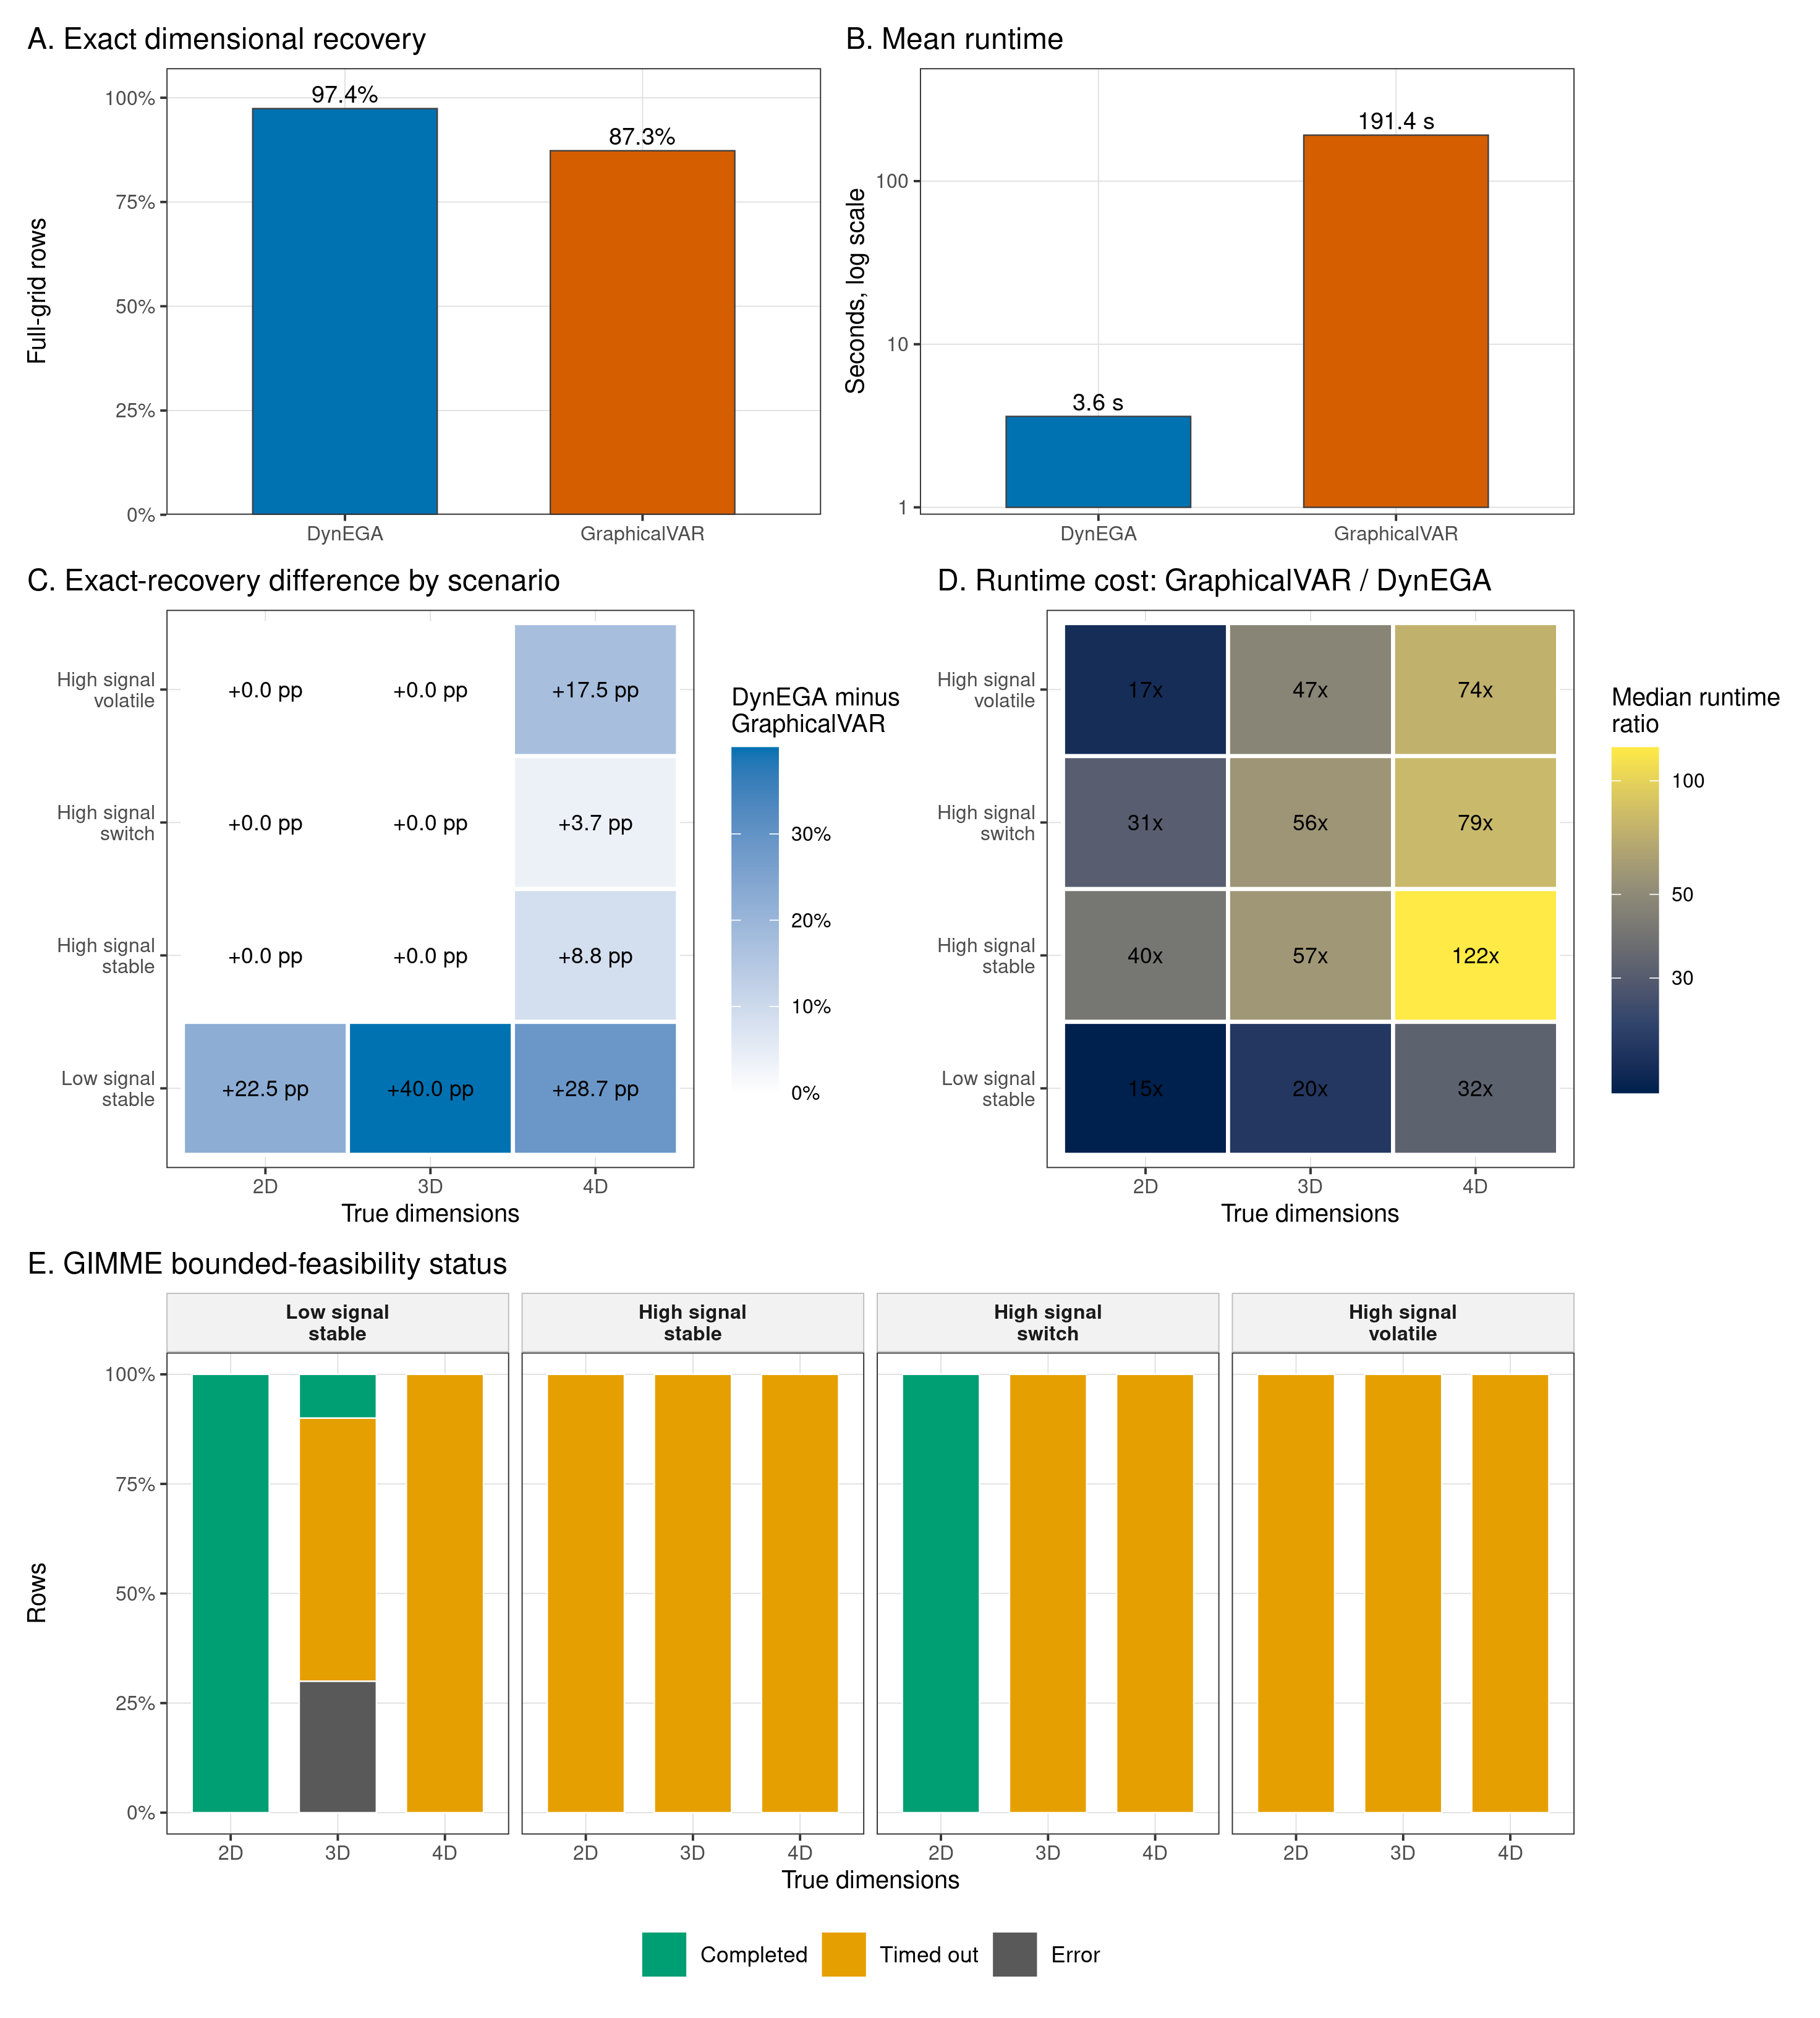
\includegraphics[width=0.98\linewidth]{comparison_revision_report_v2/benchmark_differences_v2.png}
\caption{Clean benchmark-difference summary. Panels A and B show the
method-level full-grid difference in exact dimensional recovery and runtime.
Panel C shows where DynEGA gains exact-recovery percentage points over
GraphicalVAR across scenario regimes and true dimensionality. Panel D shows the
median runtime ratio for GraphicalVAR relative to DynEGA. Panel E reports GIMME
only in its bounded feasibility role.}
\label{fig:benchmark-differences-v2}
\end{figure}

\section{OpenAI-large Empirical-Realism Check}

The OpenAI-large comparison is summarized with distributional metrics rather
than a direct visual comparison of observed and synthetic trajectories. This is
the cleaner target for the revision because the empirical question is whether
the simulator reproduces broad time-series properties, not whether a synthetic
trajectory should visually resemble any particular observed clip. The table
reports medians for the empirical OpenAI-large series and the heterogeneous DLO
simulation, together with scaled median differences and scaled distributional
distances.

\begin{table}[H]
\centering
\caption{OpenAI-large versus heterogeneous DLO metric comparison. Median
differences and distances are scaled by empirical dispersion, so smaller values
indicate a closer empirical-realism match.}
\label{tab:oai-metric-table-v2}
\small
\begin{tabular}{llrrrr}
\toprule
Family & Metric & OpenAI-large & DLO sim. & Median diff. & Distance \\
\midrule
Latent & Sample entropy & 0.427 & 0.195 & 1.08 & 0.94 \\
Latent & Lag-1 ACF & 0.567 & 0.820 & 0.90 & 0.87 \\
Latent & Standard deviation & 0.321 & 1.704 & 3.99 & 4.16 \\
Latent & Total variation & 0.179 & 0.506 & 1.81 & 1.65 \\
Latent & Zero-crossing rate & 0.214 & 0.081 & 0.96 & 0.90 \\
Raw & Sample entropy & 0.410 & 0.155 & 1.08 & 0.86 \\
Raw & Lag-1 ACF & 0.542 & 0.533 & 0.03 & 0.04 \\
Raw & Standard deviation & 0.020 & 0.077 & 1.11 & 1.17 \\
Raw & Total variation & 0.011 & 0.038 & 0.89 & 0.85 \\
Raw & Zero-crossing rate & 0.225 & 0.160 & 0.42 & 0.33 \\
\bottomrule
\end{tabular}

\end{table}

The empirical-realism evidence is mixed but useful. Raw lag-1 autocorrelation is
closely matched, and raw zero-crossing rate is reasonably close. The simulation
departs more strongly on sample entropy, standard deviation, and total
variation, with the latent score space showing larger smoothness and amplitude
mismatches. The appropriate manuscript claim is therefore not full
distributional equivalence. The better claim is that the calibrated DLO panels
capture some broad dependence properties of the OpenAI-large series while still
showing measurable departures in local irregularity and movement amplitude.

\begin{figure}[H]
\centering
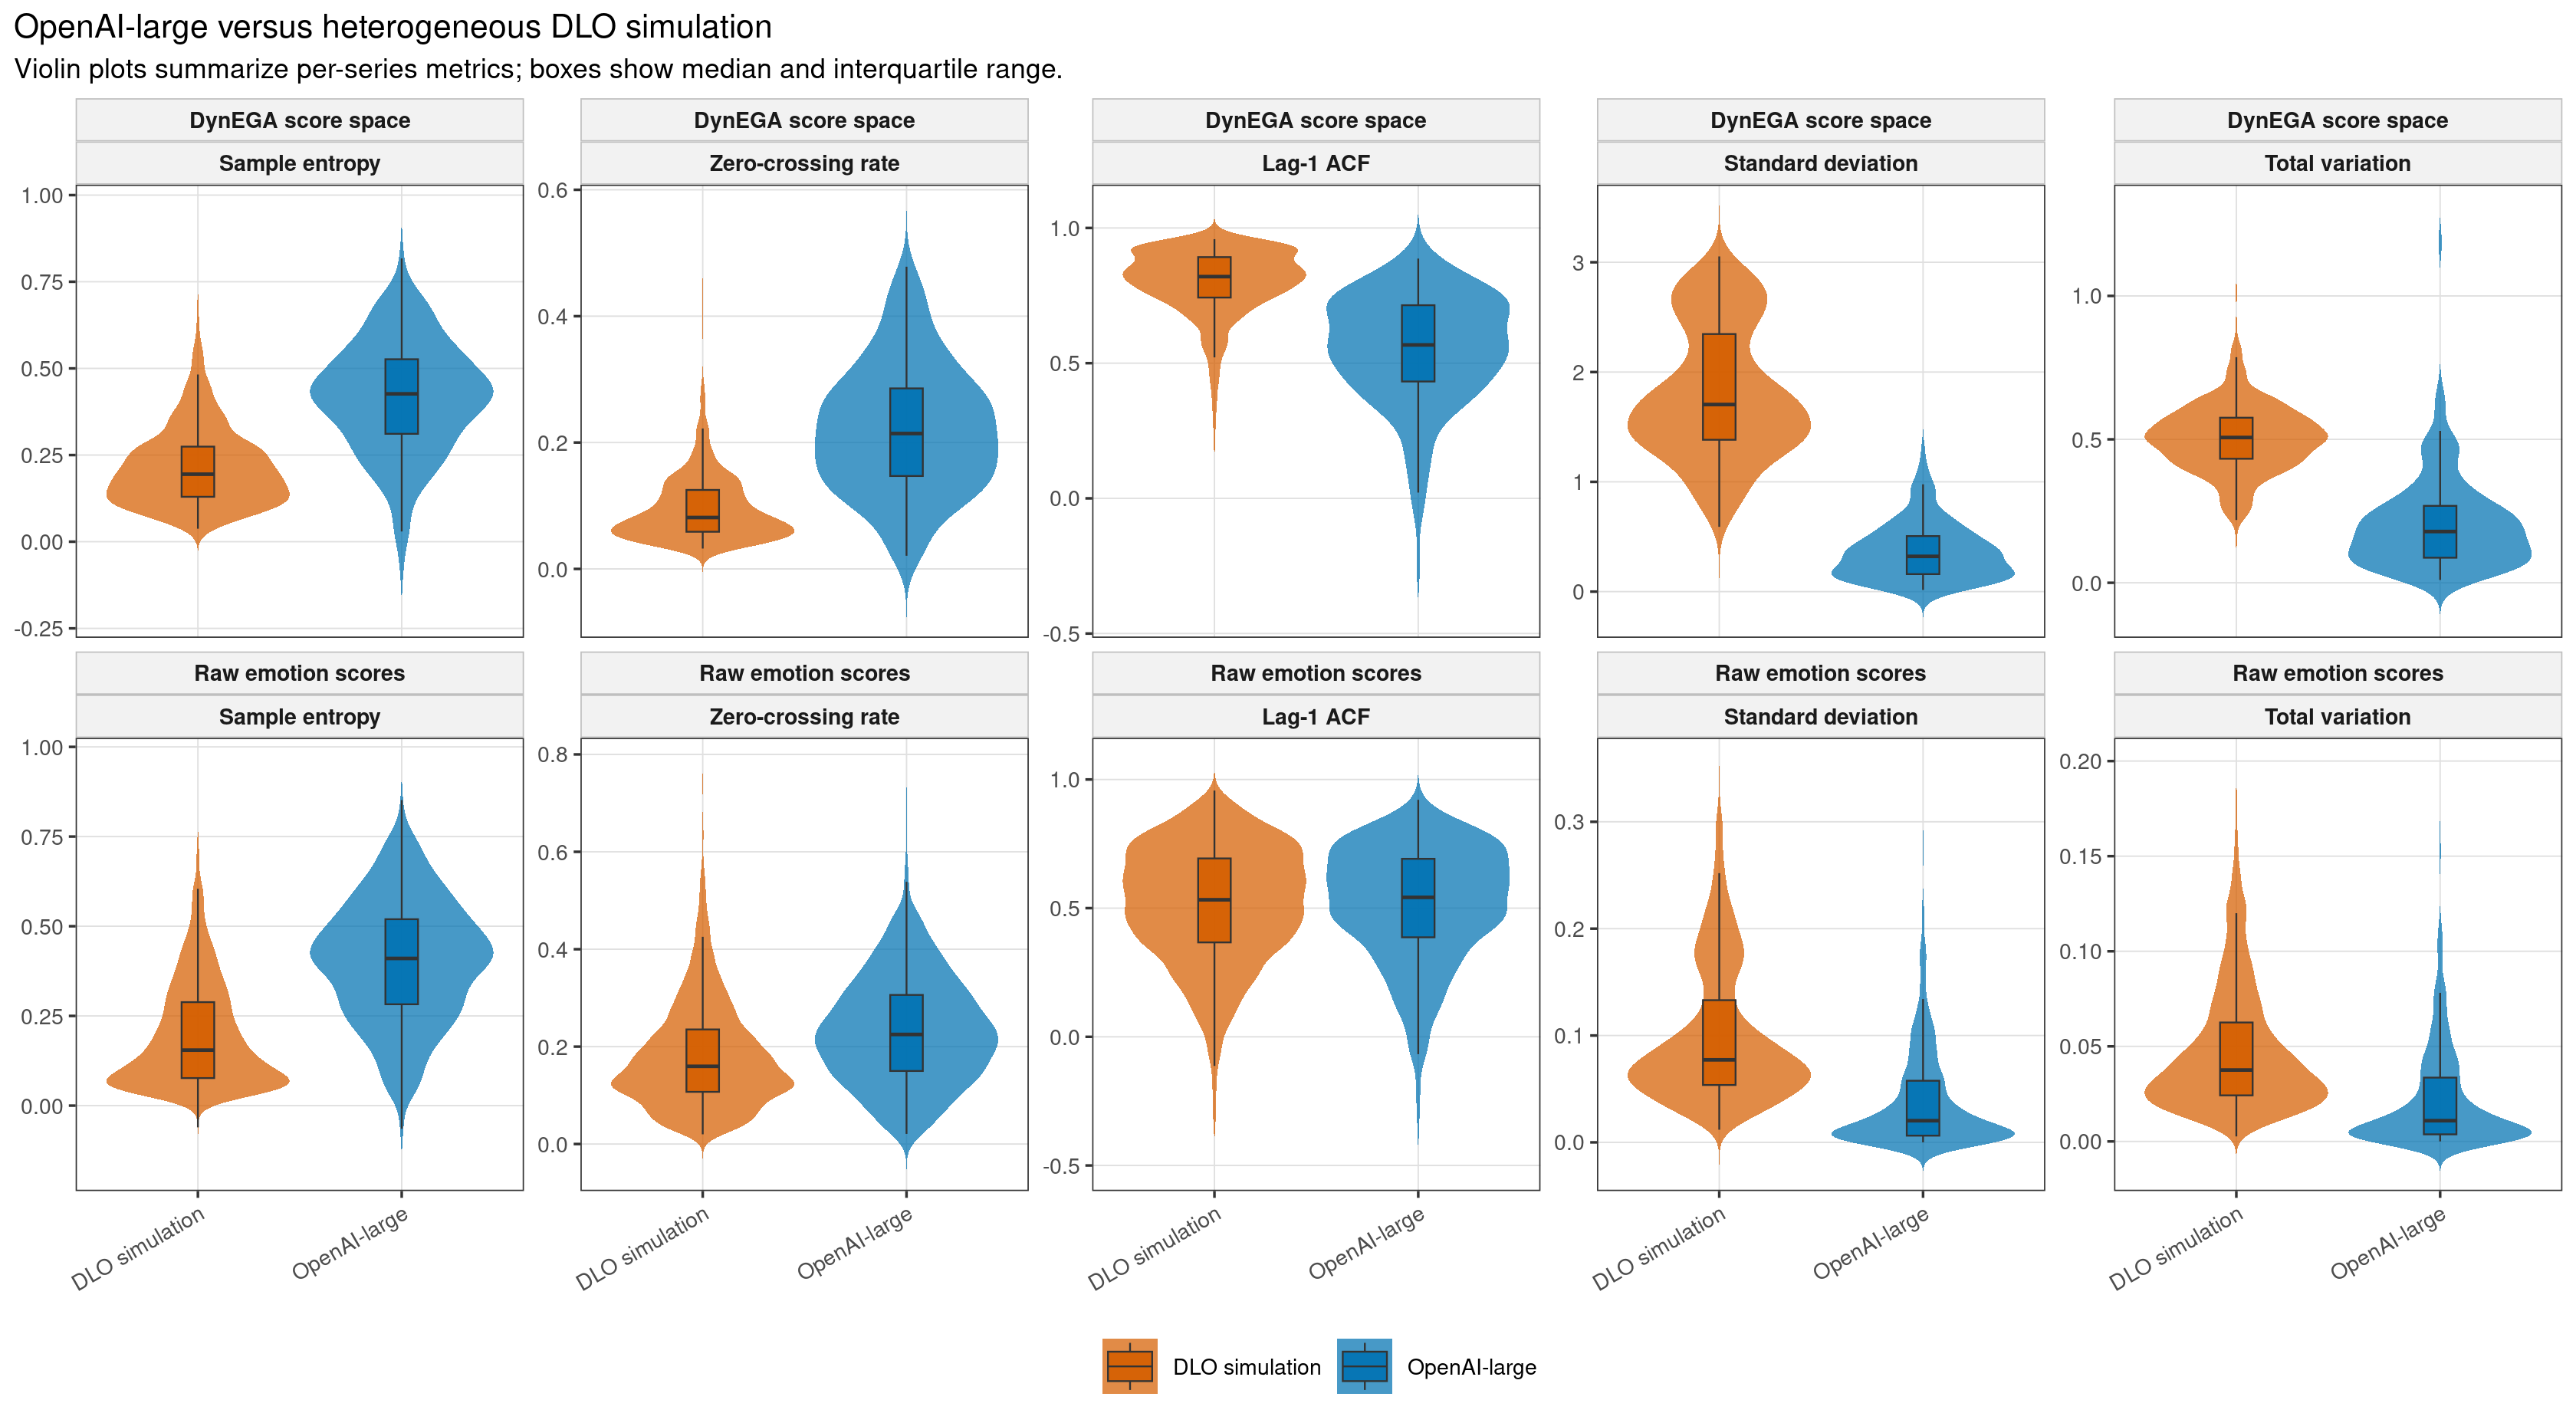
\includegraphics[width=0.98\linewidth]{comparison_revision_report_v2/oai_large_metric_violins_v2.png}
\caption{OpenAI-large versus heterogeneous DLO metric distributions. Violin
plots show per-series metric distributions for raw emotion-score series and the
DynEGA score space; embedded boxplots show medians and interquartile ranges.}
\label{fig:oai-violins-v2}
\end{figure}

\section{Benchmark Scenario Examples}

The report now uses simulated examples only to illustrate the benchmark scenario
families. These examples are not empirical comparisons. They show one simulated
two-dimensional video from each expression regime used in the benchmark, making
the distinction between low-signal stable, high-signal stable, switching, and
volatile switching scenarios visible without implying trajectory-level
correspondence to OpenAI-large clips.

\begin{figure}[H]
\centering
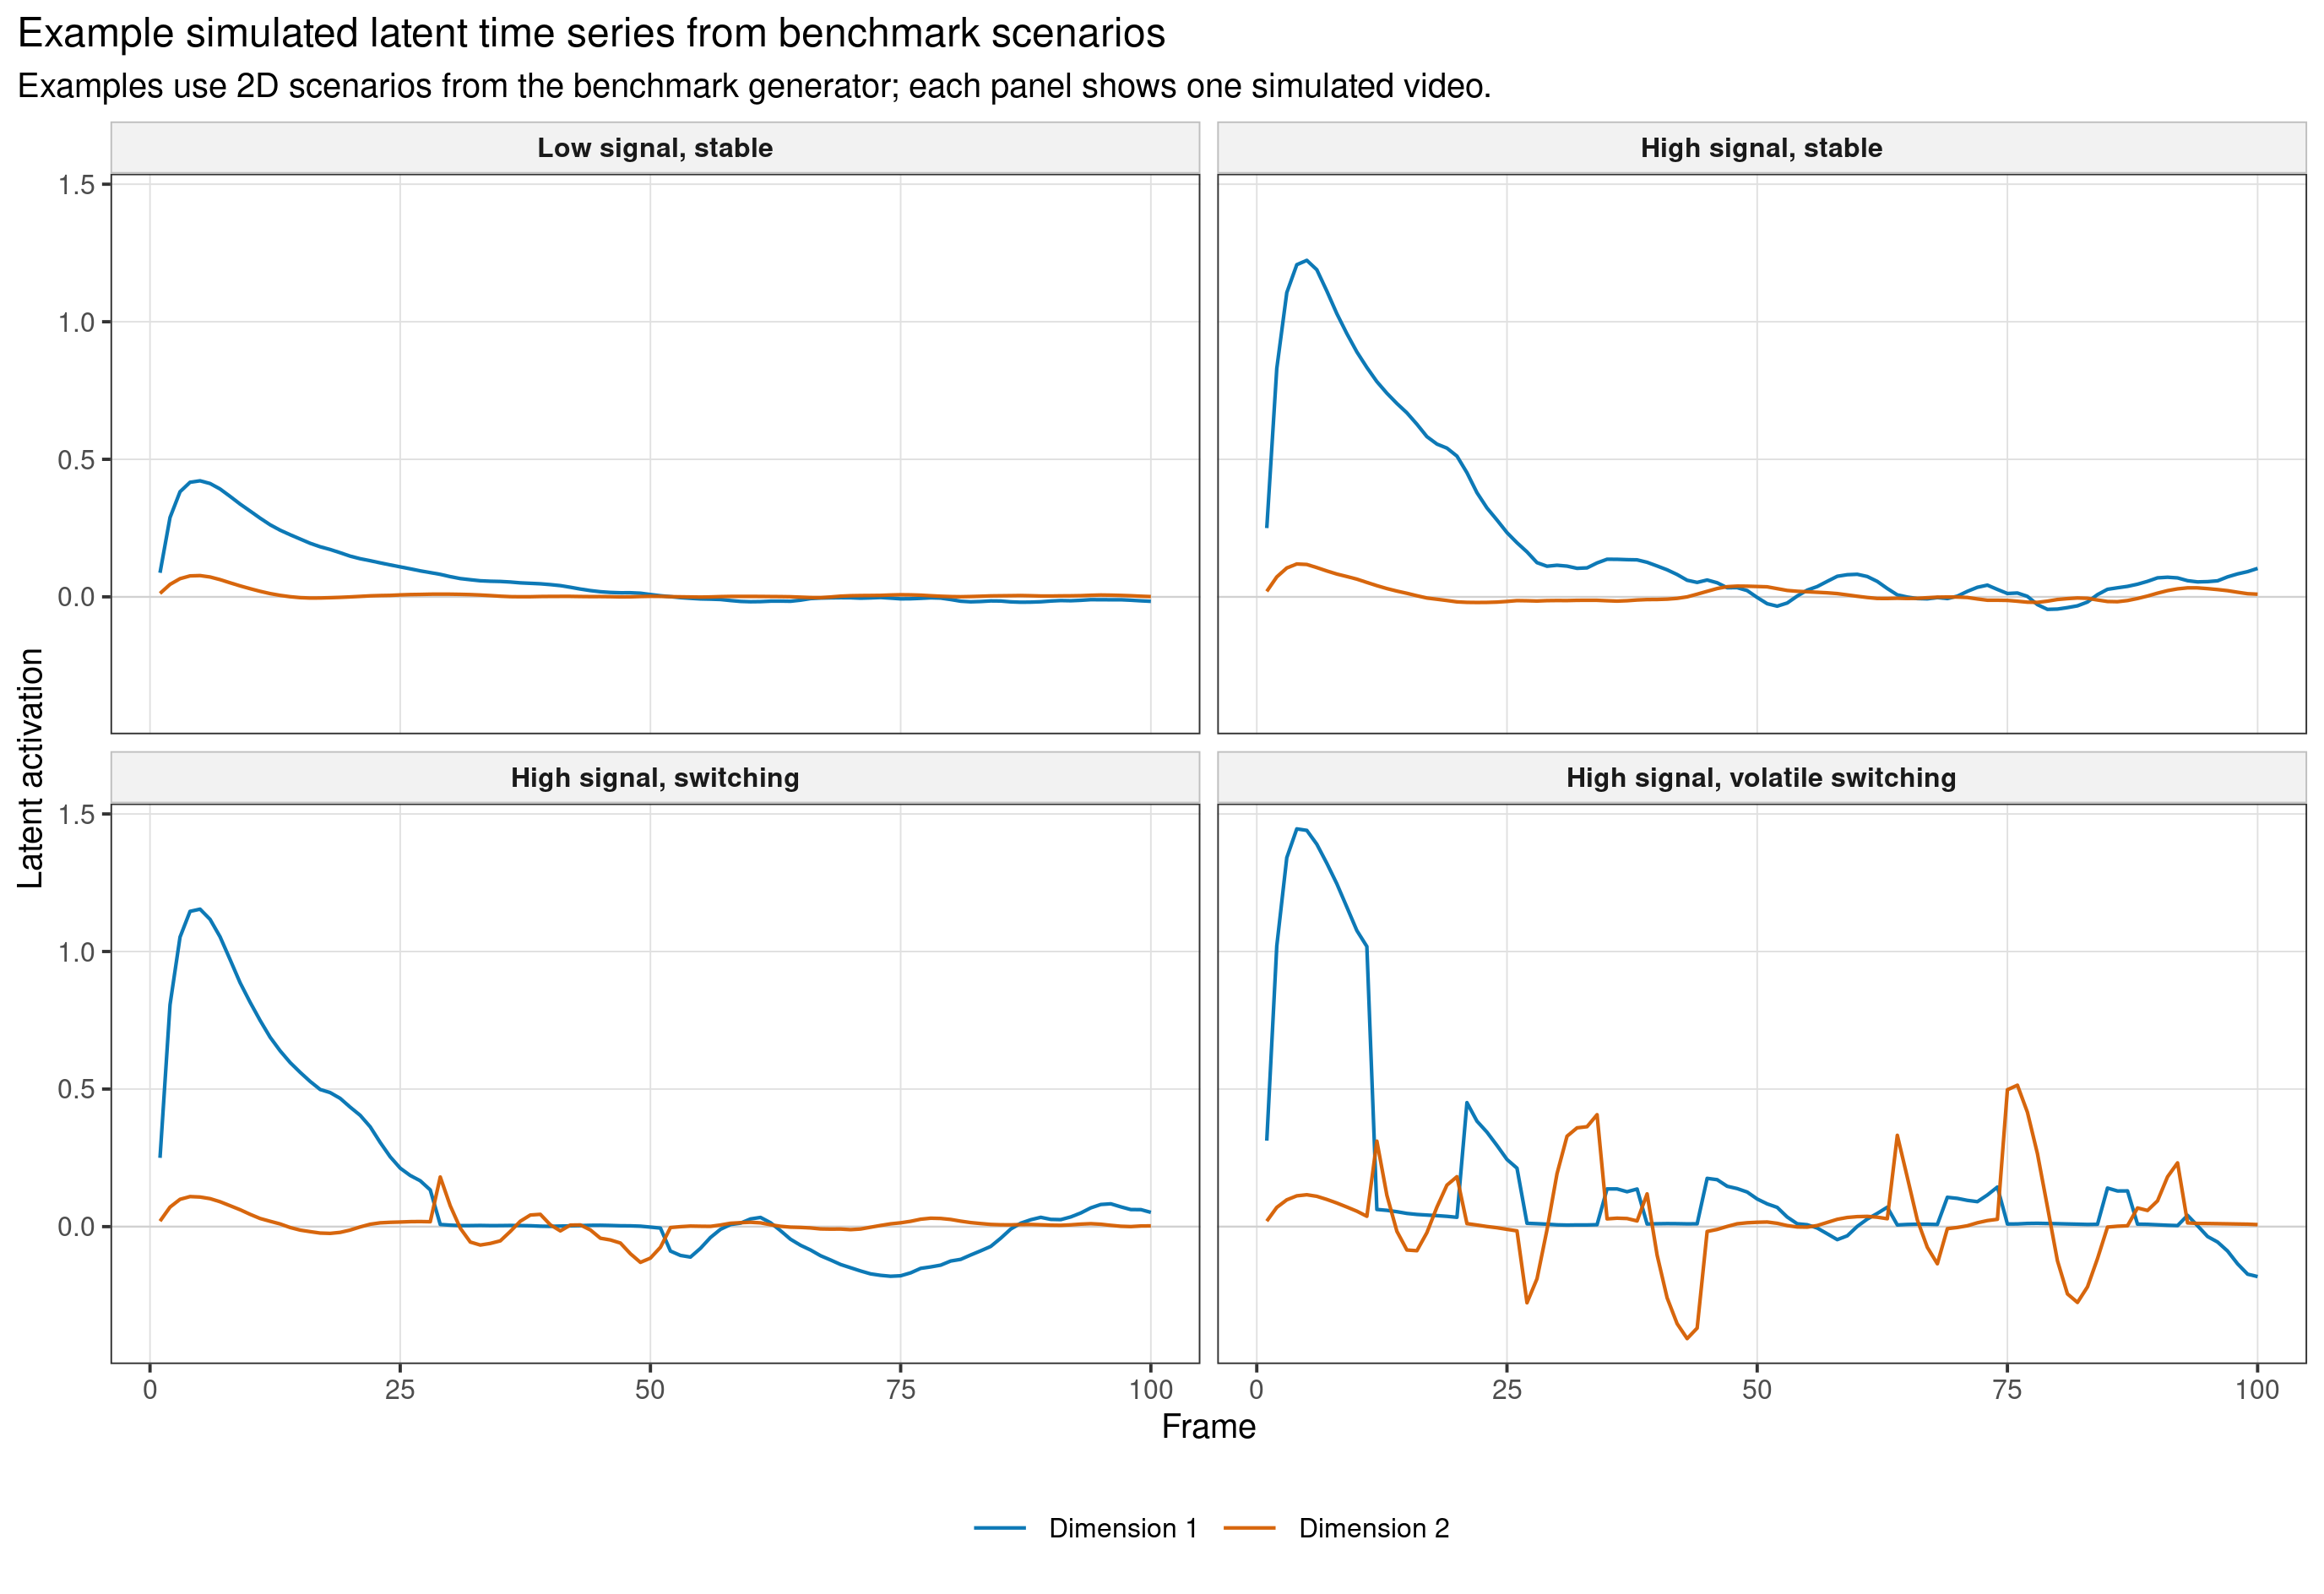
\includegraphics[width=0.95\linewidth]{comparison_revision_report_v2/benchmark_scenario_examples_v2.png}
\caption{Example simulated latent time series from the benchmark generator. Each
panel shows one two-dimensional simulated video from a benchmark scenario mode.
The figure illustrates the simulation regimes used for method recovery rather
than comparing simulated and empirical trajectories.}
\label{fig:scenario-examples-v2}
\end{figure}

\section{Revision Implications}

The revised manuscript can present DynEGA versus GraphicalVAR as the primary
benchmark result and reserve GIMME for a bounded feasibility subsection with
explicit timeout accounting. The OpenAI-large comparison should be phrased as a
metric-based realism check rather than a visual trajectory match. In writing,
the strongest defensible statement is that the current simulator is suitable for
controlled dimensional-recovery benchmarking and partially reproduces empirical
time-series structure, while remaining imperfect on entropy and amplitude
properties.

\end{document}
